
%% bare_jrnl.tex
%% V1.3
%% 2007/01/11
%% by Michael Shell
%% see http://www.michaelshell.org/
%% for current contact information.
%%
%% This is a skeleton file demonstrating the use of IEEEtran.cls
%% (requires IEEEtran.cls version 1.7 or later) with an IEEE journal paper.
%%
%% Support sites:
%% http://www.michaelshell.org/tex/ieeetran/
%% http://www.ctan.org/tex-archive/macros/latex/contrib/IEEEtran/
%% and
%% http://www.ieee.org/



% *** Authors should verify (and, if needed, correct) their LaTeX system  ***
% *** with the testflow diagnostic prior to trusting their LaTeX platform ***
% *** with production work. IEEE's font choices can trigger bugs that do  ***
% *** not appear when using other class files.                            ***
% The testflow support page is at:
% http://www.michaelshell.org/tex/testflow/


%%*************************************************************************
%% Legal Notice:
%% This code is offered as-is without any warranty either expressed or
%% implied; without even the implied warranty of MERCHANTABILITY or
%% FITNESS FOR A PARTICULAR PURPOSE! 
%% User assumes all risk.
%% In no event shall IEEE or any contributor to this code be liable for
%% any damages or losses, including, but not limited to, incidental,
%% consequential, or any other damages, resulting from the use or misuse
%% of any information contained here.
%%
%% All comments are the opinions of their respective authors and are not
%% necessarily endorsed by the IEEE.
%%
%% This work is distributed under the LaTeX Project Public License (LPPL)
%% ( http://www.latex-project.org/ ) version 1.3, and may be freely used,
%% distributed and modified. A copy of the LPPL, version 1.3, is included
%% in the base LaTeX documentation of all distributions of LaTeX released
%% 2003/12/01 or later.
%% Retain all contribution notices and credits.
%% ** Modified files should be clearly indicated as such, including  **
%% ** renaming them and changing author support contact information. **
%%
%% File list of work: IEEEtran.cls, IEEEtran_HOWTO.pdf, bare_adv.tex,
%%                    bare_conf.tex, bare_jrnl.tex, bare_jrnl_compsoc.tex
%%*************************************************************************

% Note that the a4paper option is mainly intended so that authors in
% countries using A4 can easily print to A4 and see how their papers will
% look in print - the typesetting of the document will not typically be
% affected with changes in paper size (but the bottom and side margins will).
% Use the testflow package mentioned above to verify correct handling of
% both paper sizes by the user's LaTeX system.
%
% Also note that the "draftcls" or "draftclsnofoot", not "draft", option
% should be used if it is desired that the figures are to be displayed in
% draft mode.
%
\documentclass[journal]{IEEEtran}
%
% If IEEEtran.cls has not been installed into the LaTeX system files,
% manually specify the path to it like:
% \documentclass[journal]{../sty/IEEEtran}





% Some very useful LaTeX packages include:
% (uncomment the ones you want to load)


% *** MISC UTILITY PACKAGES ***
%
%\usepackage{ifpdf}
% Heiko Oberdiek's ifpdf.sty is very useful if you need conditional
% compilation based on whether the output is pdf or dvi.
% usage:
% \ifpdf
%   % pdf code
% \else
%   % dvi code
% \fi
% The latest version of ifpdf.sty can be obtained from:
% http://www.ctan.org/tex-archive/macros/latex/contrib/oberdiek/
% Also, note that IEEEtran.cls V1.7 and later provides a builtin
% \ifCLASSINFOpdf conditional that works the same way.
% When switching from latex to pdflatex and vice-versa, the compiler may
% have to be run twice to clear warning/error messages.






% *** CITATION PACKAGES ***
%
%\usepackage{cite}
% cite.sty was written by Donald Arseneau
% V1.6 and later of IEEEtran pre-defines the format of the cite.sty package
% \cite{} output to follow that of IEEE. Loading the cite package will
% result in citation numbers being automatically sorted and properly
% "compressed/ranged". e.g., [1], [9], [2], [7], [5], [6] without using
% cite.sty will become [1], [2], [5]--[7], [9] using cite.sty. cite.sty's
% \cite will automatically add leading space, if needed. Use cite.sty's
% noadjust option (cite.sty V3.8 and later) if you want to turn this off.
% cite.sty is already installed on most LaTeX systems. Be sure and use
% version 4.0 (2003-05-27) and later if using hyperref.sty. cite.sty does
% not currently provide for hyperlinked citations.
% The latest version can be obtained at:
% http://www.ctan.org/tex-archive/macros/latex/contrib/cite/
% The documentation is contained in the cite.sty file itself.






% *** GRAPHICS RELATED PACKAGES ***
%
\ifCLASSINFOpdf
   \usepackage[pdftex]{graphicx}
  % declare the path(s) where your graphic files are
   \graphicspath{{/Users/albertocottica/github/local/communities-network-design/Pictures/}}
 
  % {{../pdf/}{../jpeg/}}
  % and their extensions so you won't have to specify these with
  % every instance of \includegraphics
  \DeclareGraphicsExtensions{.pdf,.jpeg,.png, .jpg}
\else
  % or other class option (dvipsone, dvipdf, if not using dvips). graphicx
  % will default to the driver specified in the system graphics.cfg if no
  % driver is specified.
  % \usepackage[dvips]{graphicx}
  % declare the path(s) where your graphic files are
  % \graphicspath{{../eps/}}
  % and their extensions so you won't have to specify these with
  % every instance of \includegraphics
  % \DeclareGraphicsExtensions{.eps}
\fi
% graphicx was written by David Carlisle and Sebastian Rahtz. It is
% required if you want graphics, photos, etc. graphicx.sty is already
% installed on most LaTeX systems. The latest version and documentation can
% be obtained at: 
% http://www.ctan.org/tex-archive/macros/latex/required/graphics/
% Another good source of documentation is "Using Imported Graphics in
% LaTeX2e" by Keith Reckdahl which can be found as epslatex.ps or
% epslatex.pdf at: http://www.ctan.org/tex-archive/info/
%
% latex, and pdflatex in dvi mode, support graphics in encapsulated
% postscript (.eps) format. pdflatex in pdf mode supports graphics
% in .pdf, .jpeg, .png and .mps (metapost) formats. Users should ensure
% that all non-photo figures use a vector format (.eps, .pdf, .mps) and
% not a bitmapped formats (.jpeg, .png). IEEE frowns on bitmapped formats
% which can result in "jaggedy"/blurry rendering of lines and letters as
% well as large increases in file sizes.
%
% You can find documentation about the pdfTeX application at:
% http://www.tug.org/applications/pdftex





% *** MATH PACKAGES ***
%
%\usepackage[cmex10]{amsmath}
% A popular package from the American Mathematical Society that provides
% many useful and powerful commands for dealing with mathematics. If using
% it, be sure to load this package with the cmex10 option to ensure that
% only type 1 fonts will utilized at all point sizes. Without this option,
% it is possible that some math symbols, particularly those within
% footnotes, will be rendered in bitmap form which will result in a
% document that can not be IEEE Xplore compliant!
%
% Also, note that the amsmath package sets \interdisplaylinepenalty to 10000
% thus preventing page breaks from occurring within multiline equations. Use:
%\interdisplaylinepenalty=2500
% after loading amsmath to restore such page breaks as IEEEtran.cls normally
% does. amsmath.sty is already installed on most LaTeX systems. The latest
% version and documentation can be obtained at:
% http://www.ctan.org/tex-archive/macros/latex/required/amslatex/math/





% *** SPECIALIZED LIST PACKAGES ***
%
%\usepackage{algorithmic}
% algorithmic.sty was written by Peter Williams and Rogerio Brito.
% This package provides an algorithmic environment fo describing algorithms.
% You can use the algorithmic environment in-text or within a figure
% environment to provide for a floating algorithm. Do NOT use the algorithm
% floating environment provided by algorithm.sty (by the same authors) or
% algorithm2e.sty (by Christophe Fiorio) as IEEE does not use dedicated
% algorithm float types and packages that provide these will not provide
% correct IEEE style captions. The latest version and documentation of
% algorithmic.sty can be obtained at:
% http://www.ctan.org/tex-archive/macros/latex/contrib/algorithms/
% There is also a support site at:
% http://algorithms.berlios.de/index.html
% Also of interest may be the (relatively newer and more customizable)
% algorithmicx.sty package by Szasz Janos:
% http://www.ctan.org/tex-archive/macros/latex/contrib/algorithmicx/




% *** ALIGNMENT PACKAGES ***
%
\usepackage{array}
% Frank Mittelbach's and David Carlisle's array.sty patches and improves
% the standard LaTeX2e array and tabular environments to provide better
% appearance and additional user controls. As the default LaTeX2e table
% generation code is lacking to the point of almost being broken with
% respect to the quality of the end results, all users are strongly
% advised to use an enhanced (at the very least that provided by array.sty)
% set of table tools. array.sty is already installed on most systems. The
% latest version and documentation can be obtained at:
% http://www.ctan.org/tex-archive/macros/latex/required/tools/


%\usepackage{mdwmath}
%\usepackage{mdwtab}
% Also highly recommended is Mark Wooding's extremely powerful MDW tools,
% especially mdwmath.sty and mdwtab.sty which are used to format equations
% and tables, respectively. The MDWtools set is already installed on most
% LaTeX systems. The lastest version and documentation is available at:
% http://www.ctan.org/tex-archive/macros/latex/contrib/mdwtools/


% IEEEtran contains the IEEEeqnarray family of commands that can be used to
% generate multiline equations as well as matrices, tables, etc., of high
% quality.


%\usepackage{eqparbox}
% Also of notable interest is Scott Pakin's eqparbox package for creating
% (automatically sized) equal width boxes - aka "natural width parboxes".
% Available at:
% http://www.ctan.org/tex-archive/macros/latex/contrib/eqparbox/





% *** SUBFIGURE PACKAGES ***
%\usepackage[tight,footnotesize]{subfigure}
% subfigure.sty was written by Steven Douglas Cochran. This package makes it
% easy to put subfigures in your figures. e.g., "Figure 1a and 1b". For IEEE
% work, it is a good idea to load it with the tight package option to reduce
% the amount of white space around the subfigures. subfigure.sty is already
% installed on most LaTeX systems. The latest version and documentation can
% be obtained at:
% http://www.ctan.org/tex-archive/obsolete/macros/latex/contrib/subfigure/
% subfigure.sty has been superceeded by subfig.sty.



%\usepackage[caption=false]{caption}
%\usepackage[font=footnotesize]{subfig}
% subfig.sty, also written by Steven Douglas Cochran, is the modern
% replacement for subfigure.sty. However, subfig.sty requires and
% automatically loads Axel Sommerfeldt's caption.sty which will override
% IEEEtran.cls handling of captions and this will result in nonIEEE style
% figure/table captions. To prevent this problem, be sure and preload
% caption.sty with its "caption=false" package option. This is will preserve
% IEEEtran.cls handing of captions. Version 1.3 (2005/06/28) and later 
% (recommended due to many improvements over 1.2) of subfig.sty supports
% the caption=false option directly:
%\usepackage[caption=false,font=footnotesize]{subfig}
%
% The latest version and documentation can be obtained at:
% http://www.ctan.org/tex-archive/macros/latex/contrib/subfig/
% The latest version and documentation of caption.sty can be obtained at:
% http://www.ctan.org/tex-archive/macros/latex/contrib/caption/




% *** FLOAT PACKAGES ***
%
%\usepackage{fixltx2e}
% fixltx2e, the successor to the earlier fix2col.sty, was written by
% Frank Mittelbach and David Carlisle. This package corrects a few problems
% in the LaTeX2e kernel, the most notable of which is that in current
% LaTeX2e releases, the ordering of single and double column floats is not
% guaranteed to be preserved. Thus, an unpatched LaTeX2e can allow a
% single column figure to be placed prior to an earlier double column
% figure. The latest version and documentation can be found at:
% http://www.ctan.org/tex-archive/macros/latex/base/



\usepackage{stfloats}
% stfloats.sty was written by Sigitas Tolusis. This package gives LaTeX2e
% the ability to do double column floats at the bottom of the page as well
% as the top. (e.g., "\begin{figure*}[!b]" is not normally possible in
% LaTeX2e). It also provides a command:
%\fnbelowfloat
% to enable the placement of footnotes below bottom floats (the standard
% LaTeX2e kernel puts them above bottom floats). This is an invasive package
% which rewrites many portions of the LaTeX2e float routines. It may not work
% with other packages that modify the LaTeX2e float routines. The latest
% version and documentation can be obtained at:
% http://www.ctan.org/tex-archive/macros/latex/contrib/sttools/
% Documentation is contained in the stfloats.sty comments as well as in the
% presfull.pdf file. Do not use the stfloats baselinefloat ability as IEEE
% does not allow \baselineskip to stretch. Authors submitting work to the
% IEEE should note that IEEE rarely uses double column equations and
% that authors should try to avoid such use. Do not be tempted to use the
% cuted.sty or midfloat.sty packages (also by Sigitas Tolusis) as IEEE does
% not format its papers in such ways.


%\ifCLASSOPTIONcaptionsoff
%  \usepackage[nomarkers]{endfloat}
% \let\MYoriglatexcaption\caption
% \renewcommand{\caption}[2][\relax]{\MYoriglatexcaption[#2]{#2}}
%\fi
% endfloat.sty was written by James Darrell McCauley and Jeff Goldberg.
% This package may be useful when used in conjunction with IEEEtran.cls'
% captionsoff option. Some IEEE journals/societies require that submissions
% have lists of figures/tables at the end of the paper and that
% figures/tables without any captions are placed on a page by themselves at
% the end of the document. If needed, the draftcls IEEEtran class option or
% \CLASSINPUTbaselinestretch interface can be used to increase the line
% spacing as well. Be sure and use the nomarkers option of endfloat to
% prevent endfloat from "marking" where the figures would have been placed
% in the text. The two hack lines of code above are a slight modification of
% that suggested by in the endfloat docs (section 8.3.1) to ensure that
% the full captions always appear in the list of figures/tables - even if
% the user used the short optional argument of \caption[]{}.
% IEEE papers do not typically make use of \caption[]'s optional argument,
% so this should not be an issue. A similar trick can be used to disable
% captions of packages such as subfig.sty that lack options to turn off
% the subcaptions:
% For subfig.sty:
% \let\MYorigsubfloat\subfloat
% \renewcommand{\subfloat}[2][\relax]{\MYorigsubfloat[]{#2}}
% For subfigure.sty:
% \let\MYorigsubfigure\subfigure
% \renewcommand{\subfigure}[2][\relax]{\MYorigsubfigure[]{#2}}
% However, the above trick will not work if both optional arguments of
% the \subfloat/subfig command are used. Furthermore, there needs to be a
% description of each subfigure *somewhere* and endfloat does not add
% subfigure captions to its list of figures. Thus, the best approach is to
% avoid the use of subfigure captions (many IEEE journals avoid them anyway)
% and instead reference/explain all the subfigures within the main caption.
% The latest version of endfloat.sty and its documentation can obtained at:
% http://www.ctan.org/tex-archive/macros/latex/contrib/endfloat/
%
% The IEEEtran \ifCLASSOPTIONcaptionsoff conditional can also be used
% later in the document, say, to conditionally put the References on a 
% page by themselves.





% *** PDF, URL AND HYPERLINK PACKAGES ***
%
%\usepackage{url}
% url.sty was written by Donald Arseneau. It provides better support for
% handling and breaking URLs. url.sty is already installed on most LaTeX
% systems. The latest version can be obtained at:
% http://www.ctan.org/tex-archive/macros/latex/contrib/misc/
% Read the url.sty source comments for usage information. Basically,
% \url{my_url_here}.





% *** Do not adjust lengths that control margins, column widths, etc. ***
% *** Do not use packages that alter fonts (such as pslatex).         ***
% There should be no need to do such things with IEEEtran.cls V1.6 and later.
% (Unless specifically asked to do so by the journal or conference you plan
% to submit to, of course. )


% correct bad hyphenation here
\hyphenation{op-tical net-works semi-conduc-tor}


\begin{document}
%
% paper title
% can use linebreaks \\ within to get better formatting as desired
\title{Online community management as social network design: testing for the signature of management activities in online communities}
%
%
% author names and IEEE memberships
% note positions of commas and nonbreaking spaces ( ~ ) LaTeX will not break
% a structure at a ~ so this keeps an author's name from being broken across
% two lines.
% use \thanks{} to gain access to the first footnote area
% a separate \thanks must be used for each paragraph as LaTeX2e's \thanks
% was not built to handle multiple paragraphs
%
\author{Alberto~Cottica, 
            Guy~Melan\c {c}on, 
            and Benjamin Renoust%
\thanks{Alberto is with the University of Alicante, Spain.}%
\thanks{Guy is with University of Bordeaux, France}%
\thanks{Ben is with the National Institute of Informatics \& CNRS UMI 3527 JFLI, Tokyo, Japan}%
\thanks{Manuscript last revised 2015-07-01, Draft ?please do not quote.}}

%\author{Michael~Shell,~\IEEEmembership{Member,~IEEE,}
%        John~Doe,~\IEEEmembership{Fellow,~OSA,}
%        and~Jane~Doe,~\IEEEmembership{Life~Fellow,~IEEE}% <-this % stops a space
%\thanks{M. Shell is with the Department
%of Electrical and Computer Engineering, Georgia Institute of Technology, Atlanta,
%GA, 30332 USA e-mail: (see http://www.michaelshell.org/contact.html).}% <-this % stops a space
%\thanks{J. Doe and J. Doe are with Anonymous University.}% <-this % stops a space
%\thanks{Manuscript received April 19, 2005; revised January 11, 2007.}}

% note the % following the last \IEEEmembership and also \thanks - 
% these prevent an unwanted space from occurring between the last author name
% and the end of the author line. i.e., if you had this:
% 
% \author{....lastname \thanks{...} \thanks{...} }
%                     ^------------^------------^----Do not want these spaces!
%
% a space would be appended to the last name and could cause every name on that
% line to be shifted left slightly. This is one of those "LaTeX things". For
% instance, "\textbf{A} \textbf{B}" will typeset as "A B" not "AB". To get
% "AB" then you have to do: "\textbf{A}\textbf{B}"
% \thanks is no different in this regard, so shield the last } of each \thanks
% that ends a line with a % and do not let a space in before the next \thanks.
% Spaces after \IEEEmembership other than the last one are OK (and needed) as
% you are supposed to have spaces between the names. For what it is worth,
% this is a minor point as most people would not even notice if the said evil
% space somehow managed to creep in.



% The paper headers
% \markboth{Journal of \LaTeX\ Class Files,~Vol.~6, No.~1, January~2007}%
% {Shell \MakeLowercase{\textit{et al.}}: Bare Demo of IEEEtran.cls for Journals}
% The only time the second header will appear is for the odd numbered pages
% after the title page when using the twoside option.
% 
% *** Note that you probably will NOT want to include the author's ***
% *** name in the headers of peer review papers.                   ***
% You can use \ifCLASSOPTIONpeerreview for conditional compilation here if
% you desire.




% If you want to put a publisher's ID mark on the page you can do it like
% this:
%\IEEEpubid{0000--0000/00\$00.00~\copyright~2007 IEEE}
% Remember, if you use this you must call \IEEEpubidadjcol in the second
% column for its text to clear the IEEEpubid mark.



% use for special paper notices
%\IEEEspecialpapernotice{(Invited Paper)}




% make the title area
\maketitle


\begin{abstract}
Online communities are used across several fields of human activities, as environments for large-scale collaboration. Most successful ones employ professionals, sometimes called "community managers'" or "moderators'', for a variety of tasks including onboarding new participants, mediating conflict, and policing unwanted behaviour. Network scientists routinely model interaction across participants in online communities as social networks. We interpret the activity of community managers as network design: they take action oriented at shaping the network of interactions in a way conducive to their community's goals. It follows that, if such action is successful, we should be able to detect its signature in the network itself. 

Growing networks where links are allocated by a preferential attachment mechanism are known to converge to networks displaying a power law degree distribution. Growth and preferential attachment are both reasonable first-approximation assumptions to describe interaction networks in online communities. Our main hypothesis is that managed online communities are characterised by in-degree distributions that deviate from the power law form; such deviation constitutes the signature of successful community management. If true, this hypothesis would give us with a simple test for the effectiveness of community management practices. Our secondary hypothesis is that said deviation happens in a predictable way, once community management practices are accounted for. 

We investigate the issue using empirical data on three small online communities and a computer model that simulates a widely used community management activity called \emph{onboarding}. We find that the model produces in-degree distributions that systematically deviate from power law behaviour for low-values of the in-degree; we then explore the implications and possible applications of the finding, 

\end{abstract}
% IEEEtran.cls defaults to using nonbold math in the Abstract.
% This preserves the distinction between vectors and scalars. However,
% if the journal you are submitting to favors bold math in the abstract,
% then you can use LaTeX's standard command \boldmath at the very start
% of the abstract to achieve this. Many IEEE journals frown on math
% in the abstract anyway.

% Note that keywords are not normally used for peerreview papers.
\begin{IEEEkeywords}
networks, online communities, management, power law
\end{IEEEkeywords}






% For peer review papers, you can put extra information on the cover
% page as needed:
% \ifCLASSOPTIONpeerreview
% \begin{center} \bfseries EDICS Category: 3-BBND \end{center}
% \fi
%
% For peerreview papers, this IEEEtran command inserts a page break and
% creates the second title. It will be ignored for other modes.
\IEEEpeerreviewmaketitle



%\section{Introduction}
% The very first letter is a 2 line initial drop letter followed
% by the rest of the first word in caps.
% 
% form to use if the first word consists of a single letter:
% \IEEEPARstart{A}{demo} file is ....
% 
% form to use if you need the single drop letter followed by
% normal text (unknown if ever used by IEEE):
% \IEEEPARstart{A}{}demo file is ....
% 
% Some journals put the first two words in caps:
% \IEEEPARstart{T}{his demo} file is ....
% 
% Here we have the typical use of a "T" for an initial drop letter
% and "HIS" in caps to complete the first word.
%\IEEEPARstart{T}{his} demo file is intended to serve as a ``starter file''
%for IEEE journal papers produced under \LaTeX\ using
%IEEEtran.cls version 1.7 and later.
% You must have at least 2 lines in the paragraph with the drop letter
% (should never be an issue)
%I wish you the best of success.

%\hfill mds
 
%\hfill January 11, 2007

%\subsection{Subsection Heading Here}
%Subsection text here.

% needed in second column of first page if using \IEEEpubid
%\IEEEpubidadjcol

%\subsubsection{Subsubsection Heading Here}
%Subsubsection text here.


% An example of a floating figure using the graphicx package.
% Note that \label must occur AFTER (or within) \caption.
% For figures, \caption should occur after the \includegraphics.
% Note that IEEEtran v1.7 and later has special internal code that
% is designed to preserve the operation of \label within \caption
% even when the captionsoff option is in effect. However, because
% of issues like this, it may be the safest practice to put all your
% \label just after \caption rather than within \caption{}.
%
% Reminder: the "draftcls" or "draftclsnofoot", not "draft", class
% option should be used if it is desired that the figures are to be
% displayed while in draft mode.
%
%\begin{figure}[!t]
%\centering
%\includegraphics[width=2.5in]{myfigure}
% where an .eps filename suffix will be assumed under latex, 
% and a .pdf suffix will be assumed for pdflatex; or what has been declared
% via \DeclareGraphicsExtensions.
%\caption{Simulation Results}
%\label{fig_sim}
%\end{figure}

% Note that IEEE typically puts floats only at the top, even when this
% results in a large percentage of a column being occupied by floats.


% An example of a double column floating figure using two subfigures.
% (The subfig.sty package must be loaded for this to work.)
% The subfigure \label commands are set within each subfloat command, the
% \label for the overall figure must come after \caption.
% \hfil must be used as a separator to get equal spacing.
% The subfigure.sty package works much the same way, except \subfigure is
% used instead of \subfloat.
%
%\begin{figure*}[!t]
%\centerline{\subfloat[Case I]\includegraphics[width=2.5in]{subfigcase1}%
%\label{fig_first_case}}
%\hfil
%\subfloat[Case II]{\includegraphics[width=2.5in]{subfigcase2}%
%\label{fig_second_case}}}
%\caption{Simulation results}
%\label{fig_sim}
%\end{figure*}
%
% Note that often IEEE papers with subfigures do not employ subfigure
% captions (using the optional argument to \subfloat), but instead will
% reference/describe all of them (a), (b), etc., within the main caption.


% An example of a floating table. Note that, for IEEE style tables, the 
% \caption command should come BEFORE the table. Table text will default to
% \footnotesize as IEEE normally uses this smaller font for tables.
% The \label must come after \caption as always.
%
%\begin{table}[!t]
%% increase table row spacing, adjust to taste
%\renewcommand{\arraystretch}{1.3}
% if using array.sty, it might be a good idea to tweak the value of
% \extrarowheight as needed to properly center the text within the cells
%\caption{An Example of a Table}
%\label{table_example}
%\centering
%% Some packages, such as MDW tools, offer better commands for making tables
%% than the plain LaTeX2e tabular which is used here.
%\begin{tabular}{|c||c|}
%\hline
%One & Two\\
%\hline
%Three & Four\\
%\hline
%\end{tabular}
%\end{table}


% Note that IEEE does not put floats in the very first column - or typically
% anywhere on the first page for that matter. Also, in-text middle ("here")
% positioning is not used. Most IEEE journals use top floats exclusively.
% Note that, LaTeX2e, unlike IEEE journals, places footnotes above bottom
% floats. This can be corrected via the \fnbelowfloat command of the
% stfloats package.



%\section{Conclusion}
%The conclusion goes here.





% if have a single appendix:
%\appendix[Proof of the Zonklar Equations]
% or
%\appendix  % for no appendix heading
% do not use \section anymore after \appendix, only \section*
% is possibly needed

% use appendices with more than one appendix
% then use \section to start each appendix
% you must declare a \section before using any
% \subsection or using \label (\appendices by itself
% starts a section numbered zero.)
%



\section{Introduction}

Online communities are used to aggregate and process information dispersed across many individuals. Pioneered in the 1980s, they have become more widespread with mass adoption of the Internet, and are now used across many different contexts in business \cite{mcwilliam2012building, tapscott2008wikinomics}, politics and public decision making \cite{rheingold1993virtual, noveck2009wiki, cottica2010wikicrazia}, expertise sharing \cite{rheingold1993virtual, zhang2007expertise, shirky2008here}, and education \cite{milligan2013patterns}. Most online communities lack a central command structure; despite this, many display remarkably coherent behaviour, and have proven effective at large tasks like writing the largest encyclopedia in human history (Wikipedia), providing an always-on free helpline for software engineering problems (StackOverflow), or building a detailed map of planet Earth (OpenStreetMap) \cite{shirky2008here}. 

Organizations running online communities typically employ community managers, tasked with encouraging participation and resolving conflict: this practice is almost as old as online communities themselves and predates the Internet \cite{rheingold1993virtual}, although it has become much more widespread as Internet access became a mass phenomenon. Though most participants to online communities are unpaid and answer to no one, a small number of them (only one or two in the smaller communities, many more in the larger ones) will recognize some central command, and carry out its directives. We shall henceforth call such directives \emph{policies}. 

Putting in place management policies for online communities is costly. Professional community managers need to be recruited, trained and paid; software tools to monitor communities and make their work possible need to be developed and maintained. This raises the question of why organisations running online communities choose certain policies, and not others. A full investigation of this matter is outside the scope of this paper; however, in what follows we outline and briefly discuss the set of assumptions that underpin our investigation. 

\begin{enumerate}
\item In line with the network science approach to online communities, we model online communities as social networks of interactions across participants. 
\item We assume that organisations can be modelled as economic agents maximizing some objective function. The target variable being maximized can be profit (for online communities run by commercial companies); or welfare (for online communities run by governments or other nonprofit entities); or some combination of the two. 
\item We assume that the topology of the interaction network characteristic of online communities affects their ability to contribute to the maximisation of the target variable. Indications that this assumpion might be reasonable are not difficult to find in the literature. Some examples:
\begin{itemize}
	\item When IBM decided to contribute to the development of the open source operating system Linux, it decided to unplug the project team from IBM's corporate communication network, and instructed them to adopt the communication tools of the Linux community instead. This radical reshaping of IBM's interaction network is reported to have had a great impact on the productivity of IBM programmers involved in that effort [38]. 
	\item American IT service company Geek Squad shelved their elaborate in-house design collaboration platform as their staff self-organized on an existing, third-party virtual hangout space \cite{tapscott2008wikinomics}. 
	\item Mainstream social networks like Facebook are constantly �\emph{rewiring} the interaction network across their users to ensure ever more of of them watch ever more, better targeted and more effective ads, therefore enhancing their revenue \cite{slegg2014facebook}. 
	\end{itemize}
\item We assume that such organisations choose their policies as follows: 
\begin{itemize} 
	\item Solve their maximisation problem over network topology. This yields a vector of desired network characteristics, where “desired” means that those characteristics define a maximum of the objective function. These solutions will have the form “In order to best meet our ultimate [profit or welfare] goals, the interaction network in our online community should be in state formula“, where formula is a vector of topology-related parameters.
	\item Derive a course of action that community managers could take to change the network away from its present state formulato the desired state formula.
	\item Encode such course of action in a set of simple instructions for community managers to execute. Computer scientists might think of such instructions as algorithms; economists call them mechanisms; professional online community managers call them policies. In this paper we use this third term. 
\end{itemize}
\end{enumerate}

All this implies that the decision to deploy a particular policy on an online community is very sophisticated indeed. It requires an understanding of how the shape of the interaction network within the community affects the organization's ultimate goals; therefore, to a first approximation, it can be understood as a network design exercise. And yet, interaction networks in online communities cannot really be designed; they are the result of many independent decisions, made by individuals who do not respond to the organisation's command structure. Interaction networks are, to a large extent, emergent. We conclude that an online community management policy is best understood as an attempt to “lead”, “influence”, “accompany”, “nudge” emergent social dynamics (these words are all  frequent among online community management professionals); to use a more synthetic expression, it can be best understood as the attempt to design for emergence. Its paradoxical nature is at the heart of its appeal. 

In the paper, we do not attempt to model the whole chain of decision starting from the maximization problem at step 2. Our work starts where that chain ends: we are interested in detecting the mathematical signature of one particular policy, onboarding, in the network topology. Our approach, however, does rest on the idea that organisations running online communities are trying to superimpose an element of design onto the emergent social dynamics characterizing them; that they are doing this according to a plan, which involved solving an optimisation problem; and that such plan is formulated in terms of a desired network shape. 

We consider a policy called \emph{onboarding}, perhaps one of the simplest and most common in online community management \cite{rheingold1993virtual, shirky2008here}. As a new participant becomes active (for example by posting her first post, or commenting somebody else’s post for the first time), professional community managers are instructed to leave her a comment that contains (a) friendly, positive feedback and (b) suggestions to engage with other, existing participants that she might have interests in common with. A new participants, after her first contribution, would get a comment like this by one of the moderators:

\emph{``Welcome, Alice! That was a very interesting point. It definitely resonates with my own experience in the field. In our community, the people who are most involved in the matter are Bob [link] and Charlie [link]. You might be interested in this post [link] by Bob, where he relates his own experience: if you leave him a comment, I am sure an interesting conversation will ensue.''}

If the new participant engages (by replying or asking a question), she gets another message (an acknowledgement or an answer); after that, the new participant is generally considered onboarded, and is not made the object of any special attention.

This paper considers the issue of why organizations running online communities invest considerable resources in onboarding, and how can they determine whether their investment has been productive. We do so by modeling online conversations as social networks of interactions across participants, and looking for the effect that onboarding has on the topology of those networks.

Section 2 briefly examines the two strands of literature that we mostly draw upon. Section 3 presents some data from real-world online communities; then proceeds to describe our main experiment, based on a computer simulation of interaction in online communities with and without onboarding. Section 4 presents the experiment's results. Section 5 discusses them.

\section{Literature survey}

The extraordinary successes of online communities in deploying large-scale, decentralized projects has led many scholars to conjecture that online communities exhibit emergent behavior, and called such behavior collective intelligence, after an influential book by Pierre L\'evy \cite{pierre1997collective}. This name was adopted by a research community that aims at providing tools for better collective sense- and decision making such as argument maps (representations of the logical structure of a debate, with all redundancy eliminated) \cite{shum2003roots} and attention-mediation metrics (indicators that signal what, in an online debate, is worthiest reading and responding to. The number of Likes on Facebook is one such metric) \cite{klein2012enabling}. 

Collective intelligence scholars acknowledge the existence and importance of online community management practices – indeed, they have tried for some time to systematize it \cite{blondel2008fast, diplaris2011emerging} and produce technological innovation to support it \cite{de2012contested}. An important part of their research program aims to better equip community managers to carry out this work; for example, argument maps are advocated on the basis that the effort to build them will engage more users in the debate, and will do so more effectively than competing engagement techniques \cite{shum2003roots}. These tools are meant to facilitate and encourage participation to online communities, to make it easier for individuals to extract knowledge from them.

Starting in the 2000s, online communities became the object of another line of enquiry, stemming from network science. Network representation of relationships across groups of humans has yielded considerable insights in social sciences since the work of the sociometrists in the 1930s, and continues to do so; phenomena like effective spread of information, innovation adoption, and brokerage have all been addressed in a network perspective \cite{borgatti2009network, burt2009structural}. As new datasets encoding human interaction became available, many online communities came to be represented as social networks. This was the case for social networking sites, like Facebook \cite{lewis2008tastes, nick2013toward}; microblogging platform like Twitter \cite{kunegis2013preferential, java2007we, hodas2014simple}; news-sharing services like Digg \cite{hodas2014simple}; collaborative editing projects like Wikipedia \cite{laniado2011wikipedians}; discussion forums like the Java forum \cite{zhang2007expertise}; and bug reporting services for software developers like Bugzilla \cite{zanetti2012quantitative}). Generally, such networks represent participants as nodes. Edges represent a relationship or interaction which varies according to the nature of the online community in question: friendship for Facebook; follower-followed relationship, retweet or mention in Twitter; vote or comment in Digg and the Java forum; talk in Wikipedia; comment in Bugzilla. 

In contrast to collective intelligence scholars, network scientists typically do not address the issue of community management, and treat social networks drawn from online interaction as fully emergent. In this paper, we employ a network approach to investigate the issue of whether the work of community managers leaves a footprint detectable by quantitative analysis, and of what kind. By doing so, we seek to make community management practices easier and more accountable to monitor, with a view of making online communities better at achieving their goals, be them maintaining an encyclopedia or collectively writing a new constitution. 

In particular, we exploit a result from the theory of evolving networks. This substantial branch of the literature on networks originates from seminal work by Barabási and Albert \cite{barabasi1999emergence} in 1999. Departing from previous network theory work, they observe that most networks in nature grow over time, with new nodes adding themselves to the network; and that new nodes do normally not connect to existing nodes with equal probability, but rather prefer to link to nodes that are already highly connected. They then show that the assumption of growth and preferential attachment, when taken together, result in a network whose degree distribution converges to a power law: 

This result holds for any network that displays growth and preferential attachment, and the exponent is shown to be analytically equal to 3 \cite{barabasi2005origin, barabasi1999mean}.  The model was later generalized by Dorogovtsev and Mendes to allow for non-preferential attachment to coexist with preferential attachment; new edges forming between existing nodes; and for some nodes to be more attractive than others. The generalized model was shown to converge to a power law with exponent ranging from 2 to infinity. This prediction was confirmed across a broad range of networks, including many social networks \cite{dorogovtsev2002evolution}.

With a view to this goal, we propose that Dorogovtsev and Mendes result \cite{dorogovtsev2002evolution} holds for interaction in online communities, too. More explicitly, we assume that the network representing interaction in an online community, left to its own device – in the absence of community management policies, will converge to a degree distribution that follows a power law with exponent 2 or larger. We then use this prediction as a baseline state. A policy successfully enacted on the online community, with community managers being instructed to execute certain tasks, will result in its degree distribution deviating from the baseline power law in predictable ways. Such deviation can be interpreted as the signature that the policy is working well. 

The most important one difficulty in this method is the absence of a counterfactual: if a policy is enacted in the online community, the baseline degree distribution corresponding to the absence of the policy is not observable, and viceversa. This rules out a direct proof that the policy “works”. Instead, we proceed as follows: 

\begin{enumerate}
\item We initially examine data from three small online communities. Two of them deploy an active policy to welcome new members and integrate them with the incumbent ones (a practice sometimes called onboarding), while the third one does not. We observe that, indeed, the shape of the degree distribution of the first two differs from that of the third.  
\item We propose an experiment protocol to determine whether onboarding policies can explain the differences observed between the degree distributions of the first two online communities and that of the third one. 
\item We simulate the growth of online communities by means of a computer model. Variants to the model cover the relevant cases: the absence of onboarding policies and their presence, with varying degrees of effectiveness. 
\item We run the experiment protocol against the degree distributions generated by the computer model, and discuss its results.
\end{enumerate}
\section{Material and methods}

In this section we introduce the empirical data, the experiment protocol and the simulation model we use in the experiment. 

\subsection{Empirical data}

We examine data from three real-world online communities. All three use the same software (Drupal 7), are roughly comparable in size and are used by practitioners and interested citizens to publicly discuss issues that have a collective dimension. They are modeled as interaction networks, in which nodes are registered users and edges represent comments. The presence of an edge from Alice to Bob indicates that Alice has commented content authored by Bob at least once. The resulting graphs are directed (“Alice comments Bob” is not equivalent to “Bob comments Alice” and weighted (Alice can write multiple comments to Bob's content; the edge's weight is equal to the number of comments written). Table 1 presents some descriptive statistics about them. 

\begin{itemize}
\item \emph{InnovatoriPA} is a community of (mostly) Italian civil servants discussing how to introduce and foster innovation in the public sector. It does not employ any special onboarding or moderation policy.
\item \emph{Edgeryders} is a community of (mostly) European citizens, discussing public policy issues from the perspective of grassroot activism and social innovation. It adopts a policy of onboarding new members.
\item \emph{Matera 2019} is a community of (mostly) citizens of the Italian city of Matera and the surrounding region, discussing the city's policies as it made a bid to be appointed European Capital of Culture 2019. It adopts a policy of onboarding new members.
\end{itemize}


\begin{table*}[t]
\centering 
\begin{tabular}{| c | c | c | c |} 
\hline 
& Innovatori PA & Edgeryders & Matera2019\\ 
& \emph{``no special policy''} & \emph{``onboard new users''} & \emph{``onboard new users''}\\ 
\hline 
In existence since & December 2008 & October 2011 & March 2013 \\
Accounts created & 10,815 & 2,419 & 512 \\
\hline 
Active participants (nodes) & 619 & 596 & 198 \\
Number of edges (weighted) & 1,241 & 4,073 & 883 \\
\hline 
Average distance3 & 3.77 & 2.34 & 2.51 \\
Maximum degree & 155 & 238 & 46 \\
Average degree & 2.033 & 6.798 & 4.454 \\
\hline 
\% nodes with $d_+(n) = 0$ & 0.657 & 0.138 & 0.227 \\
\% nodes with $d_+(n) = 1$ & 0.141 & 0.159 & 0.182 \\
\% nodes with $d_+(n) = 2$ & 0.065 & 0.125 & 0.121 \\
\% nodes with $d_+(n) > 2$ & 0.137 & 0.579 & 0.470 \\
\hline 
\end{tabular}
\caption{Comparing interaction networks three online communities}
\label{tab:template}
\end{table*}



We fit power laws in-degree distributions of these three online communities, as of early December 2014. Next, we tested the hypothesis that degree distributions follow a power law, as predicted by the theory. This was done in the following way:
\begin{enumerate}
\item first, we fitted power functions to the entire support of each in-degree distribution, i.e. for any degree greater than or equal to 1. 
\item next, we fitted power functions to the right tail of each in-degree distribution, i.e. for any degree greater than or equal to, where formulais the degree that minimizes the Kolmogorov-Smirnov distance between the fitted function and the data with in-degree formula.
\item finally, we ran goodness-of-fit tests for each in-degree distribution and for fitted power functions as described in both 1 and 2. The null hypothesis tested is that the observed distribution is generated by a power function with exponentformula. We used a test based on comparing the Kolmogorov-Smirnov D statistic of the observed distribution with those of a large number of synthetic datasets drawn by the fitted power function. Such comparison is summarized in a p-value, that indicates the probability of the D statistic to exceed the observed value conditional to the null hypothesis being true. Observing p-values close to 1 indicate that the power function is a good fit for the data, and do not allow rejection of the null hypothesis; p-values close to zero indicate that the power function is a bad fit for the data, and lead to to reject the null hypothesis. The rejection value is set, conservatively, at 0.1.  The method we followed is borrowed from Clauset, Shalizi and Newman \cite{champernowne1953model} and is described in detail in the Appendix. 
\end{enumerate}
	
We emphasize in-degree, as opposed to out-degree, for the following reason. The Barabási-Albert model and many of its extensions \cite{dorogovtsev2002evolution} have been applied to undirected as well as to directed network. However, directedness is implicit in the idea of preferential attachment. When networks are directed, it is reasonable to expect the in-degree distribution to be the one to follow a power law. This expectation has been confirmed by empirical investigation \cite{klein2012enabling}, supporting the conjecture that some preferential attachment is present in many in online conversation networks. As new members join, many of them will reach out to someone, and it seems to make sense that they will target highly connected individuals more. 

Results are summarized in Table 2. 

\begin{table}[b]
\centering 
\begin{tabular}{| c | c | c | c |} 
\hline 
&  &  & $p$-value\\ 
\hline 
Innovatori PA & 1.611 & 1 & 0.21 \\
formula & & & \\
\hline
Edgeryders & 1.477 & 1 & 0.00 - \emph{reject} \\
formula & & & \\
\hline
Edgeryders & 2.250 & 5 & 0.45 \\
formula & & & \\
\hline
Matera2019 & 1.506 & 1 & 0.00 - \emph{reject} \\
formula & & & \\
\hline
Matera2019 & 2.817 & 6 & 0.94 \\
formula & & & \\
\hline 
\end{tabular}
\caption{Testing for goodness-of-fit of power functions to interaction networks of degree distributions in three online communities.}
\label{tab:goodnessoffit}
\end{table}

As we consider the interval formula, we find that the in-degree distribution of the Innovatori PA interaction network – the unmoderated one – is consistent with the expected behavior of an evolving network with preferential attachment; we cannot reject the null hypothesis that it was generated by a power law. The same is not true of the other two online communities – both with onboarding policies – for which the null hypothesis is strongly rejected.  

When we consider only the tail of the degree distributions, i.e. degree distributions for formula, on the other hand, all three communities display a behavior that is consistent with that of evolving networks with preferential attachment.

This set of results is consistent with the objectives of the onboarding policy. These consist of helping newcomers to overcome the initial difficulties associated with finding your way around an online community that they don't know yet. A successfully onboarded new user will generally have some extra interaction with existing community members with respect to ones that are left to themselves; all things being equal, we can expect this to lead to extra edges appearing in the interaction network, and interfering with the in-degree distribution that would appear in the absence of onboarding. This could explain the non-power law in-degree distribution of Edgeryders and Matera2019. On the other hand, it is reasonable to expect this interference to concern mostly low connectivity nodes: onboarding targets predominantly newcomers, and focuses on helping them through the first few successful interactions. Highly active (therefore highly connected) community members do not need to be onboarded. This could explain why, when we consider only the highly connected nodes in the distribution's upper tails, all three communities display similar behavior, regardless of onboarding policies. 

\subsection{Experiment protocol}
The difference observed between the two communities with onboarding policies and the one without might be caused not by the policy itself, but by some other unobserved variable. To explore the issue further, we generate and compare computer simulations of interaction networks in online communities that are identical except for the presence and effectiveness of onboarding policies. Communities are assumed to grow over time, with new participants joining them in sequence; at each point in time, new edges appear; their probability of targeting an existing node grows linearly with that node's in-degree. Additionally, communities might have or not have onboarding policies. If they do have them, their effectiveness is summarized by a scalar that varies from 0 to 1 and can be interpreted as the probability that the community manager's onboarding action will have the desired effects. We specify the precise meaning of both onboarding actions and their desired effects in the next section.

We proceed as follows.

First, we simulate the evolution of the interaction network of a large number of online communities. Divide them into a control group (no onboarding policy) and a treatment group (presence of onboarding policy). Specifically, we simulate the evolution of the interaction network of:

\begin{itemize}
\item 100 communities with no onboarding policy. These will constitute the control group of our simulated communities. 
\item 100 communities with an onboarding policy characterized byformula(ineffective onboarding). 
\item 100 communities with an onboarding policy characterized by.
\item 100 communities with an onboarding policy characterized byformula. 
\item 100 communities with an onboarding policy characterized byformula. 
\item 100 communities with an onboarding policy characterized byformula. 
\item 100 communities with an onboarding policy characterized byformula(fully effective onboarding). All communities with some form of onboarding, even if ineffective, are included in the treatment group.
\item For each of these networks, we compute the in-degree distribution.
\end{itemize}

Next, we define the following hypotheses. 

\begin{itemize}
\item Let C be the network of interaction in an online community. Denote the in-degree of nodes in the network byformula. Let P be the best-fit power-law model for the in-degree distribution of C.
\item \emph{Hypothesis 1}. The in-degree distribution of C is generated by P for any formula.
\item \emph{Hypothesis 2}. The in-degree distribution of C is generated by P for any formula, where formulais the in-degree that minimizes the Kolmogorov-Smirnov distance between the fitted function and the data over formula.
\end{itemize}

Finally, we test Hypothesis 1 and 2 on each of the 1400 in-degree distributions generated. We do this using the goodness-of-fit tests proposed by Clauset et.al. \cite{clauset2009power} and illustrated in detail in the Appendix.
We expect to obtain the following:

\begin{itemize}
\item In the control group, both Hypothesis 1 and Hypothesis 2 are true. 
\item In the treatment group with fully effective onboarding Hypothesis 1 is false and Hypothesis 2 is true. 
\item In the intermediate situations of partially ineffective onboarding, Hypothesis 1 can be true or false, according to the value of formula. Hypothesis 2 is true.
\end{itemize}


\subsection{The simulation model}

Our computer model simulates the growth of an interaction network in an online community with and without onboarding.  

\subsubsection*{Without on boarding}

We use the model without onboarding to generate the networks in our control group. Its growth mechanism for the network to grow is based on preferential attachment, consistently with the Barabási-Albert tradition. We follow the more general formulation of Dorogovtsev and Mendes \cite{dorogovtsev2002evolution}.
\begin{itemize}
\item A network is initialized, consisting of two reciprocally connected nodes
\item At each time step, one new node – representing a participant in the online community – appears in the network. 
\item At each time step,  new edges – representing comments – appear in the network. The source of each edge is drawn at random from the uniform distribution of the existing nodes4. Its target is chosen according to the following rule: the probability that the new edge points to node s is proportional to where formulais a parameter representing additional attractiveness of the node.
\end{itemize}

\subsubsection*{With on boarding}

We use a variant of the above model that includes onboarding to generate the networks in our treatment group. The variant consists simply of the model without onboarding, to which further steps are added.
\begin{itemize}
\item At each timestep, one edge is directed towards the newcomer node. This is meant to represent the community manager's onboarding action described in section 1. 
\item At each timestep, with probability formula, one edge is added. Its source is the newcomer node; its target is chosen according to the following rule: the probability that the new edge points to node s is proportional to formulawhere formulais a parameter representing additional attractiveness of the node. This is meant to represent the newcomer's reaction to the community manager's onboarding activity; as a result of the latter, the newcomer becomes active and reaches out to someone in the community, as advised by the community manager. We assume that community managers will normally incline to point newcomers to existing users who are reputed to be interesting conversationalists, and that the characteristic of being interesting conversationalists is correlated with node in-degree. [nu1] can be thought of as representing onboarding effectiveness. More skilled community managers will be more persuasive in inducing newcomers to reach out and engage in the conversation taking place in the online community.
\item At each timestep, with probability one edge is added. Its source is drawn at random from the uniform distribution of the existing nodes; its target is the newcomer node. This represents a successful onboarding outcome: the new participant, by becoming active, has attracted the attention of some existing participant, who has engaged with her. The new participant, no longer isolated, is now in conversation.
\item For the purpose of the present paper, we set and we let formula
\end{itemize}


\section{Results}
Following the protocol outlined in section 3.2, we evolved 100 networks for each of the seven variants of the model. For all networks, we set network size to 2000 nodes; ; and . These choices are discussed in the appendix.

\subsection{Goodness-of-fit of the power-law model}

For each network evolved we computed two best-fit power-law models, one for formulaand the other for formulawhere formulais the in-degree the minimizes the Kolmogorov-Smirnov distance between the fitted function and the data over formula. On each of these models , we ran a goodness-of-fit test as described in section 3.2. This resulted in two distributions of p-values for our control group, plus two more for each of our six treatment groups. Table 3 and 4 report descriptive statistics for these distributions.

Table 3: Testing for goodness-of-fit of power-law models to degree distributions of interaction networks in online communities, with no onboarding and with onboarding. The parameter formula approximates the effectivess of the onboarding action. Power-law models are estimated over all nodes with degree formula.

From Table 3, we conclude that onboarding seems to have some effect on the goodness-of-fit of the generated data to their respective best-fit power-law models when formula. The effect goes in the direction of reducing the p-values. The rightmost column counts the networks for which the goodness-of-fit test returns a p-value below 0.1 (the threshold value below which the literature recommend Hypothesis 1 is rejected), out of the 100 runs. 

It is useful to address the question of whether Hypothesis 1 can be rejected in the aggregate, rather than for each individual network. We can do so by computing T-tests on the null hypothesis that the average p-value in each case is equal to 0.1, against an alternate hypothesis of p-value being smaller than 0.1. The results of such tests are summarized in Table 4.

Table 4: Testing for mean p-values equal to 0.01. The second column reports the value of the t statistic; the third column reports the probability of the alternate hypothesis mean < 0.1 being true. 0.1 is the threshold value below which our hypothesis H1 is rejected, as recommended by \cite{clauset2009power}. Power-law models are estimated over all nodes with in-degree formula.

Illustration 1 shows the cumulate density functions of the p-values in the control and treatment groups. 

Illustration 1: Cumulate Density Functions of p-values for each of the seven batches of networks. 20\% of the networks evolved without onboarding (dark blue) have degree distributions that test negatively for H1. When onboarding is introduced, that percentage rises to between 50 and 90%. A higher effectiveness of onboarding reduces the number of rejections. Power-law models are estimated over all nodes with degree formula.

When we consider only the upper tail of the in-degree distribution (formula), the effect of introducing onboarding on the goodness-of-fit is much less clear. All but 13 networks generated display scaling behavior in the upper tail when formula is chosen so as to minimize the Kolmogorov-Smirnov distance between the generated data and the best-fit power-law model. We conclude that we do not reject Hypothesis 2, regardless of whether onboarding is present or not. 

OLE-objectTable 5: Testing for goodness-of-fit of power-law models to in-degree distributions of interaction networks in online communities, with no onboarding and with onboarding. The  parameter approximates the effectivess of the onboarding action. Power-law models are estimated over all nodes with in-degree formula , where formula is the value that minimized the Kolmogorov-Smirnov distance between the fitted power-law model and the empirical data.

\subsection{Lower bounds}
Our results show a limited, albeit statistically significant, effect of onboarding on the value of formula, the value of formula that minimizes the Kolmogorov-Smirnov distance between the data generated by the computer simulation and the best-fit power-law model. Table 6 illustrates, for each batch of 100 networks, the average value of formula, its standard error and the  result of a t-test on the null hypothesis that formulavs the alternate hypothesis that formula, where denotes the effectiveness of the onboarding activity. 

OLE-objectTable 6: Testing the null hypothesis that formula Introducing onboarding has the effect to increase formula, the value that minimized the Kolmogorov-Smirnov distance between the fitted power-law model and the empirical data. This effect is statistically significant at the 5% level for , and at the 0.1% level for formula.

Illustration 2: Cumulate Density Functions of the degrees at which networks exhibit power law behaviour, for each of the seven batches of networks generated. A little over 60% of the networks evolved without onboarding (dark blue) approximate power-law models best when such power-law models are fitted with lower bound 3 or lower. When onboarding is introduced, that percentage decreases to between 20 and 50%.  

\begin{figure}[thb]
\centering

	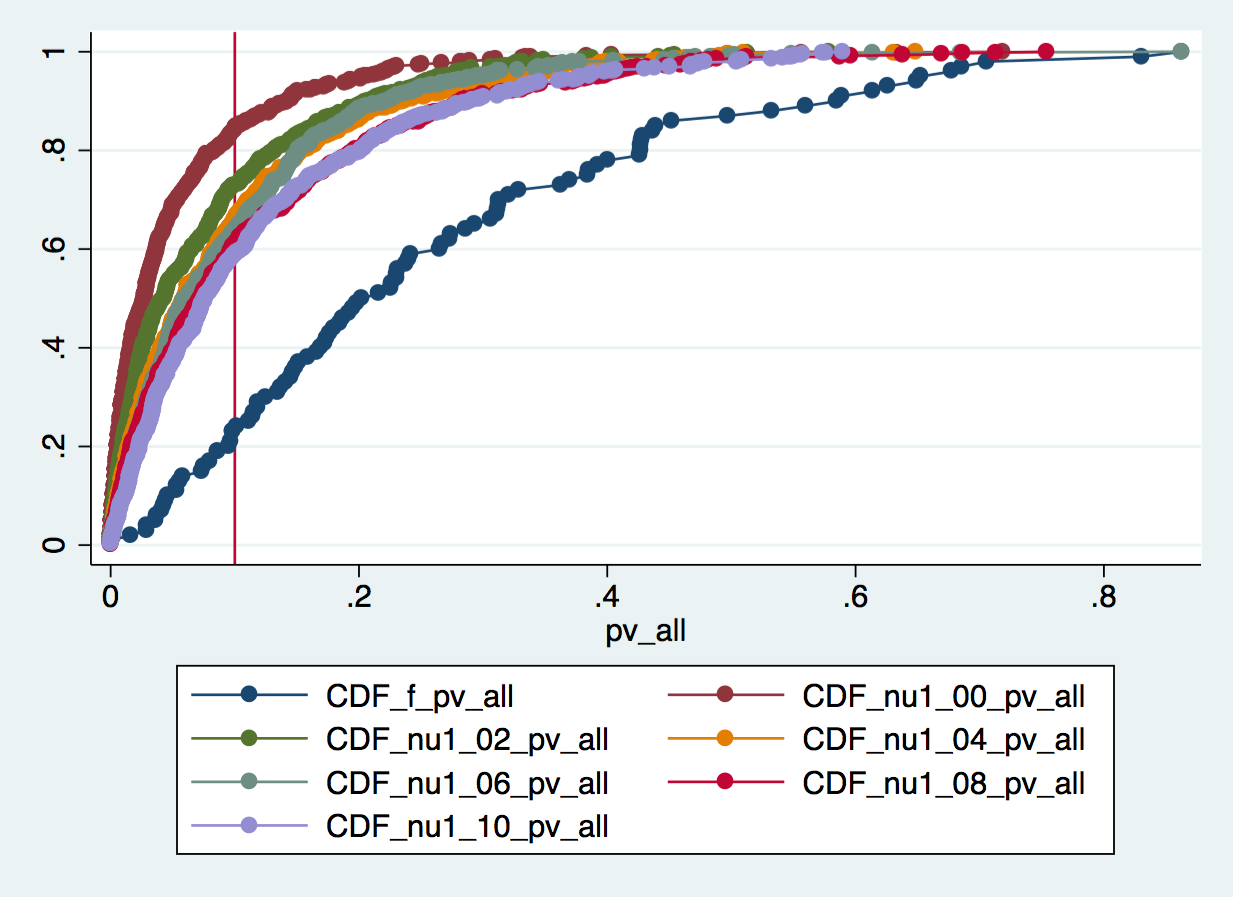
\includegraphics[width=.9\linewidth]{../Pictures/CDF_nu1.png}\label{fig:CDFnu1}
	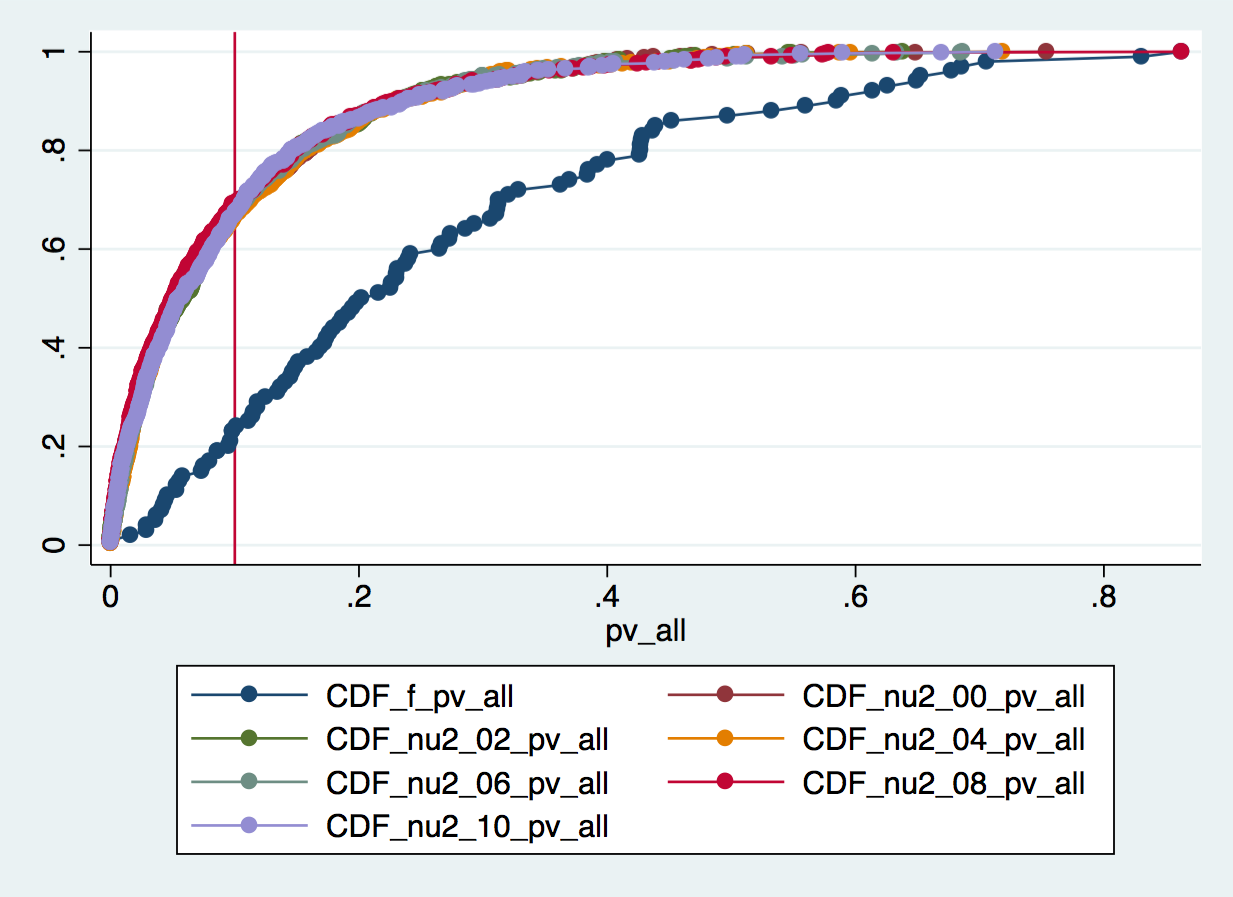
\includegraphics[width=.9\linewidth]{../Pictures/CDF_nu2.png}\label{fig:CDFnu2}
  %\subfloat[][]{}
  %\subfloat[][]{}
  \caption{Influence of parameters $\nu_1$ an $\nu_2$}
 \label{fig:CDF}
\end{figure}


\subsection{Exponents}
When considering only the tails of the in-degree distributions (formula), we find that introducing onboarding has a positive and significant on the value of the exponent. This is consistent with the theoretical results by Dorogovtsev and Mendes \cite{dorogovtsev2002evolution}, who proved that introducing a fraction of non-preferential attachment edges in evolving networks with preferential attachment does not suppress the power-law dependence of its degree distribution, but only increases the scaling exponent thereof. Table 7 summarizes the results of t-tests on the null hypothesis that formula against the alternative hypothesis that formula, where is the scaling exponent. 

OLE-objectTable 7: Testing the null hypothesis that   for different levels of onboarding effectiveness. When a p-value of 0.05 is set as the rejection threshold, the null hypothesis is rejected in favor of the alternative hypothesis that formulafor all values of the effectiveness parameter. When a p-value of 0.01 is chosen instead, the null hypothesis is rejected in favour of the alternative hypothesis in all cases, save for .
\section{Discussion}

\subsection{Accounting for degree distribution shape in the interaction networks of online communities}

Our simulation model incorporates two forces. The first one is preferential attachment; the second is onboarding. The former is meant to represent the rich-get-richer effect observed in many real-world social networks; the latter is meant to represent the onboarding action of moderators and community managers. The former's effect is known to lead to the emergence of an in-degree distribution that approximates a power-law model. The latter's effect is more subtle, because it is in turn composed of two effects. The first one consists in the direct action of the moderator, which  always targets the newcomer; the second one by the actions that might be undertaken as a result of well-executed onboarding policy. 

The direct action of the moderators creates edges pointing to nodes not selected by preferential attachment – this is definitional of online community management. What (non-moderator) participants in the online community do as a result of moderator activity is not as clear cut. In our simulation model, fully successful onboarding results in extra edges, some of which point to nodes selected by preferential attachment, others to nodes selected otherwise. 

Also, onboarding only targets newcomers in online communities. As most of online community management policies, it concerns weakly connected participants in the community: moderators have no need to engage with very active, strongly connected participants, who clearly need no help in getting a conversation going. By doing so, moderators hope to help some shy newcomers turn into active, respected, sought out community members. Once this process is under way, however, moderators have no reason to continue to engage with the same individuals. In terms of our model, this means that newcomers, after having being onboarded, are going to receive new edges by preferential attachment only. It is therefore reasonable to expect that the degree distributions generated by our model display a heavy tail, with the frequency of highly connected nodes following a reasonable approximation of a power law. The overall result of onboarding, then, is an in-degree distribution with power-law behavior for high values of formula and non-power law behavior for low (close to 1) values of formula. This is indeed what we observe. 

Non-preferential attachment selection of edge targets leads to a poorer fit of power-law models to the in-degree distributions of the interaction networks of online communities where onboarding is present. This effect takes two forms. The first one is that, when onboarding is present, fitting a power-law model to the network's in-degree distribution and then running goodness-of-fit tests return a lower p-value than the p-value returned by the same test when onboarding is absent. The second effect is that, with onboarding, the value of formulathat minimizes the Kolmogorov-Smirnov distance between the best-fit power-law model and the observed data tends to be higher than without onboarding.

Our specification of the model accounts for an apparent paradox: the deviation of the observed networks' degree distributions from power-law behaviour is greater when onboarding is present, but completely ineffective. Ineffective onboarding only adds edges directly created by moderators, none of which are allocated across existing nodes by preferential attachment. As onboarding gets more effective, even more edges are added; some are allocated by preferential attachment, and drive the degree distribution back towards a pure power-law behavior. 

\subsection{Limitations}

We undertook this research work in the hope of discovering a simple test that could be used to assess the presence and effectiveness of online community management policies, onboarding among them. The guiding idea is that the agency of online community managers and moderators is guided by a logic other than the rich-get-richer dynamics that spontaneously arises in many social networks. Such dynamics is associated to power-law shaped degree distributions, which we can regard as the default state for social interaction networks: we conjecture that, whenever the interaction network of an online community does not have the shape of a power law, some agency is at work. We furthermore conjecture that the precise nature of such deviations can be interpreted, and ultimately that different social forces at work on an online community each leave their different mathematical signatures on the community's interaction network. Such signatures could, in principle, be read in the precise form of the deviation of the degree distribution from its default state. 

Our results are in accordance with the first conjecture. Applying onboarding to our simulated community, in whatever form, results in degree distributions that are markedly more distant from pure power-law behavior than we find in our control group. However, we do not find a monotonic relationship between onboarding's effectiveness and the distance of the resulting degree distribution from a pure power-law form. When we observe real-world online community whose interaction networks do not have a full power-law form (like those of Section 3.1); even though we are informed that they do employ onboarding policies; and even if we knew that onboarding policies are the only factor likely to affect the patterns of interaction within those communities, we could still not conclude from the form of their degree distributions how effective these policies are. 

The high dimensionality of the problem space is also a limitation. As stylized as it is, our model has several parameters interacting in complex ways: the number of edges generated at each time step, the additional attractiveness parameter, the probability that the newcomer reacts to the onboarding action, and the probability that such reaction attracts the attention of some other participant, that engages in conversation with the newcomer. This problem is compounded by the model's nontrivial computational intensity. 

\subsection{Directions for future research}

There are three obvious directions in which our work could be taken further. The most obvious one is a full and systematic exploration of the parameter space, with the goal of assessing our results' robustness with respect to model specification. In this paper we restrict ourselves to the presence and effectiveness of the onboarding action in a baseline model which is closely modeled on Dorogovtsev's and Mendes's results [16]; it would be useful to test for how these results carry through as we alter other parameters of the model, such as the number of edges  created at each time step, the additional attractiveness parameter . In the same vein, we would gain analytical granularity by resolving the effectiveness parameter  into its components  and .

A second direction for further research would be to attempt to make the model into a more realistic description of a real-world online community. Such an attempt would draw attention onto how some real-world phenomena, when incorporated in the model, influence its results. It would also carry the advantage of allowing online community management professional to more easily interact with the model and critique it. Several issues that could be investigated in this vein come to mind. For example, we could relax the assumption that the additional attractiveness parameter formula is identical for all nodes, allowing for different nodes in the network to attract incoming edges at different rates (a phenomenon known as multiscaling [6]). Secondly, we could introduce a relationship between out-degree and in-degree: this would reflect the fact that , in an online community, reaching out to others (which translates in increasing one's own out-degree in the interaction network) is a good way to get noticed and attract incoming comments (which translates in an increas in one's in-degree). Thirdly, we could work with online community manager professionals to model more precisely the action of online community managers: in this paper we assume that community managers recommend newcomers to reach out to existing participants, targeting with higher probability those with higher in-degrees; alternatives could be considered, for example uniformly random allocation or, in a model with multiscaling, targeting with higher probability participants with higher attractiveness. Finally, we could extend the model to consider not only onboarding, but other community management policies as well. Again, this would require close cooperation with online community management professionals.

A third direction for further research would attempt to gauge the influence of onboarding and other community management policies on network topology by indicators other than the shape of its degree distribution, such as the presence of subcommunities. 



\appendices

\section{Appendix}
\subsection{Testing for goodness-of-fit of a power law distribution}

The goodness-of-fit tests we employed were built following a procedure indicated by Clauset, Shalizi and Newman \cite[pp. 15-18]{clauset2009power}. What follows summarizes it in the context of the paper. The test's null hypothesis is that the empirical data are distributed according to a power law model; the alternative hypothesis is that they are not.

First, we fit the data for the degree distribution of a network generated by our model to a discrete power-law model, using maximum likelihood estimation. When we are testing for goodness-of-fit of the entire degree distribution, we set the fitted power-law model lower bound to 1; when we are testing for goodness-of-fit of the distribution's upper tail only, we choose a lower bound  such that the Kolmogorov-Smirnov distance $D$ between the power law model and the empirical data is minimized. Formally, define

\[D = \underset_{k>=k_{min}{max}} | S(k) - P(k)| \]

Here, $S(k)$ is the cumulative density function of the data for the observations with value at least $k_{min}$, and $P(k)$ is the cumulative density function for the power-law model that best fits the data in the region $k>=k_{min}$. The value of $k_{min}$ that minimizes the function $D$ is the estimate for the model's lower bound.

Next, we generate a large number of power-law distributed synthetic datasets with the same scaling parameter, standard deviation and lower bound as those of the distribution that best fits the empirical data. We fit each of these synthetic datasets to its own power-law model and calculate the $D$ statistics of each one relative to its own model. Finally, we count what fraction of the values of $D$ thus computed is larger than the value of $D$ computed for the empirical data. This fraction is interpretable as a p-value: the probability that data generated by our estimated best-fit power-law model will be more distant from the model than our empirical data (``distant'' in the Kolmogorov-Smirnov sense). A p-value close to zero indicates that it is quite unlikely that the estimated power-law model would generate empirical data so distant from the fitted power function; a p-value close to one, on the contrary, indicates that the estimated power model is quite likely to generate empirical data that are further away from the fitted power function than the ones we collected. 

Generating artificial datasets requires a treatment for the region below $k_{min}$  that differs from that of the one above it. We proceed as follows. Assume that our observed dataset has $n$ observations total and $n_{tail}$ observations such that $k>=k_{min}$. To generate a synthetic datasets with $n$ observations, we repeat the following procedure $n$ times:
\begin{itemize}
\item With probability $n/n_{tail}$ we generate a random number $k_i$ with $k_i>=k_{min}$, drawn from a power law with the same scaling parameter as our best-fit model.
\item Otherwise, with probability $1 - n/n_{tail}$, we select one element uniformly at random from among the elements of the observed dataset in the region $k<k_{min}$.
\end{itemize}

At the end of the process, we will have a synthetic dataset that follows the estimated power-law model for $k>=k_{min}$, but has the same non-power law distribution below $k_{min}$.

This test requires we decide how many synthetic datasets to generate for each test; and what is the threshold value below which we reject the null hypothesis. Again based on \cite{clauset2009power} we make the following decisions:

\begin{itemize}
\item We set the number of artificial datasets generated to 2500. This corresponds to an accuracy of about 0.01, based on an analysis of the expected worst-case performance of the test. 
\item We conservatively set the rejection threshold at 0.01.
\end{itemize}

\subsection*{A2. Choosing parameter values}

The computer simulation's computational intensity prevented us from conducting a thorough exploration of its behaviour across the whole parameter space. It follows we had to pick values from some parameters. In this section we discuss briefly our choice of parameter values.
The choice of $m=1$ implies that the number of edges in the networks in our control group will be equal to the number of nodes; we initialize the network with two nodes connected by two edges (one in each direction), then add one node and one edge at each time step. A glance at  Figure \ref{fig:NetViz} shows that this is unrealistic. The real-world online communities described in section 3.1 all display a number of edges with is a multiple of the number of nodes. We justify this choice as follows: in a real-world thriving online community there are many things going on at any given time. Both the spontaneous activities of its participants and the command-and-control work of online community managers and moderators follow multiple logics. 
 
In the paper, we are interested in pitting against each other two of these logics, that of preferential attachment, that tends to generate rich-gets-richer phenomena; and that of onboarding, that tends to introduce a measure of equality. The way we modeled onboarding is by having one single incoming edge targeting the only newcomer to the community at each timestep; we therefore chose to have one single non-onboarding generated edge at each timestep. It seems reasonable that our choice would make  these two forces roughly equivalent to each other, and make the impact of onboarding on the in-degree distribution easier to detect.

The choice of $A=1$ follows from another, and more fundamental, modeling choice. We mimic Dorogovtsev's and Mendes's approach, where the network being modeled is directed and the probability of a new edge to target a node with in-degree $k$ is proportional to $k$ \cite{dorogovtsev2002evolution}; this contrasts with Barab\'asi's and Albert's approach, that models the network as undirected and assumes that the probability of a new edge to target a node is proportional to its total degree. In a Dorogovtsev-Mendes type model, new nodes have, by construction, in-degree zero, whereas in a Barab\'asi-Albert type model new nodes have total degree one. It follows that, in a Dorogovtsev-Mendes type model, the parameter $A$ tunes the "traction"�� of preferential attachment: the higher its value, the weaker the grip of pure preferential attachment. For $A=0$ Dorogovtsev-Mendes type models degenerate into "multiple star networks", where the probability of newcomers to receive an edge is zero, and all edges target the nodes initially in the network for all time. 

Setting $A = 1$ we make the probability of a newcomer to receive its first edge equal to one half that of an incumbent participant who already has one incoming edge to receive its second one, one third of that of an incumbent participant who already has two incoming edges to receive its third one and so on. One can check that this behaviour mimics that of the simplest, and best known, Barab\'asi-Albert type model. 

\subsection*{A.3 Software stack}

To obtain the results discussed in the paper we made use of the following software applications:
\begin{itemize}
\item Graphs were handled through the networkx Python library.
\item Parallel computation was handled through the multiprocessing Python package. 
\item The estimation of power-law models and the generation of synthetic data made use of the PowerLaw Python package developed by Alstott et al. \cite{alstott2014powerlaw}.
\item The network visualizations were drawn with Edgesense: https://github.com/Wikitalia/edgesense
\end{itemize}


\section*{Acknowledgements}
The authors gratefully acknowledge the invaluable contributions of Giovanni Ponti, Raffaele Miniaci, Noemi Salantiu, Lee-Sean Huang, the faculty and students at University of Alicante and everybody at Masters of Networks 3.

Alberto Cottica acknowledges the support of the CATALYST European project in developing the Edgesense tool and acting as a conversation starter between the collective intelligence and the network science research communities.




%\section{Proof of the First Zonklar Equation}
%Appendix one text goes here.

% you can choose not to have a title for an appendix
% if you want by leaving the argument blank
%\section{}
%Appendix two text goes here.


% use section* for acknowledgement
%\section*{Acknowledgment}


%The authors would like to thank...


% Can use something like this to put references on a page
% by themselves when using endfloat and the captionsoff option.
\ifCLASSOPTIONcaptionsoff
  \newpage
\fi



% trigger a \newpage just before the given reference
% number - used to balance the columns on the last page
% adjust value as needed - may need to be readjusted if
% the document is modified later
%\IEEEtriggeratref{8}
% The "triggered" command can be changed if desired:
%\IEEEtriggercmd{\enlargethispage{-5in}}

% references section

% can use a bibliography generated by BibTeX as a .bbl file
% BibTeX documentation can be easily obtained at:
% http://www.ctan.org/tex-archive/biblio/bibtex/contrib/doc/
% The IEEEtran BibTeX style support page is at:
% http://www.michaelshell.org/tex/ieeetran/bibtex/
%\bibliographystyle{IEEEtran}
% argument is your BibTeX string definitions and bibliography database(s)
%\bibliography{IEEEabrv,../bib/paper}
%
% <OR> manually copy in the resultant .bbl file
% set second argument of \begin to the number of references
% (used to reserve space for the reference number labels box)
\bibliographystyle{IEEEtran}
\bibliography{bibliography}

%\end{document}

%\begin{thebibliography}{1}

%\bibitem{IEEEhowto:kopka}
%H.~Kopka and P.~W. Daly, \emph{A Guide to \LaTeX}, 3rd~ed.\hskip 1em plus
%  0.5em minus 0.4em\relax Harlow, England: Addison-Wesley, 1999.

%\end{thebibliography}

% biography section
% 
% If you have an EPS/PDF photo (graphicx package needed) extra braces are
% needed around the contents of the optional argument to biography to prevent
% the LaTeX parser from getting confused when it sees the complicated
% \includegraphics command within an optional argument. (You could create
% your own custom macro containing the \includegraphics command to make things
% simpler here.)
%\begin{biography}[{\includegraphics[width=1in,height=1.25in,clip,keepaspectratio]{mshell}}]{Michael Shell}
% or if you just want to reserve a space for a photo:

\begin{IEEEbiography}{Alberto Cottica}
Biography text here.
\end{IEEEbiography}

% if you will not have a photo at all:
%\begin{IEEEbiographynophoto}{John Doe}
%Biography text here.
%\end{IEEEbiographynophoto}

% insert where needed to balance the two columns on the last page with
% biographies
%\newpage

%\begin{IEEEbiographynophoto}{Jane Doe}
%Biography text here.
%\end{IEEEbiographynophoto}

% You can push biographies down or up by placing
% a \vfill before or after them. The appropriate
% use of \vfill depends on what kind of text is
% on the last page and whether or not the columns
% are being equalized.

%\vfill

% Can be used to pull up biographies so that the bottom of the last one
% is flush with the other column.
%\enlargethispage{-5in}



% that's all folks
\end{document}


